\documentclass{extbook}
\usepackage[papersize={8.5in,11in},top=1in,bottom=1in]{geometry}
\RequirePackage{fix-cm}
\usepackage[T1]{fontenc}
\usepackage{lmodern}
\usepackage{fullpage}
\usepackage{titlesec}
\usepackage{parskip}
\usepackage{float}
\usepackage{url}
\usepackage{hyperref}
\usepackage{graphicx}
\usepackage{tcolorbox}
\usepackage{tabularx}
\usepackage{xcolor}
\usepackage{titlesec}
\usepackage{amsmath}
\usepackage{tcolorbox}
\usepackage{tabularx}

\renewcommand{\contentsname}{Contenido}
\renewcommand{\figurename}{Figura}
%\renewcommand{\listtablename}{Lista de tablas}
\renewcommand{\listfigurename}{Lista de figuras}
\usepackage[fontsize=13.5pt]{fontsize}
\setlength{\parindent}{0pt}

\titleformat{\chapter}[display]
  {\bfseries\huge} % Estilo del título
  {\hfill\Large} % Alineación a la derecha
  {3ex} % Espaciado entre el número del capítulo y el título
  {\vspace{-5cm}\titlerule\vspace{1.5ex}\hfill} % Regla arriba y alineación del título a la derecha
  [\vspace{1ex}\titlerule] % Regla debajo del título


  \makeatletter
  \patchcmd{\chapter}
    {\if@openright\cleardoublepage\else\clearpage\fi}
    {\clearpage}
    {}{}
  \makeatother

  \definecolor{codegreen}{rgb}{0,0.6,0}
  \definecolor{codegray}{rgb}{0.5,0.5,0.5}
  \definecolor{codepurple}{rgb}{0.58,0,0.82}
  \definecolor{backcolour}{rgb}{0.95,0.95,0.92}

\begin{document}
\begin{titlepage}
  \begin{center}
      {\huge \textbf{Universidad Tecnológica de Panamá}}\\
      \vspace{3mm}
      {\Large \textbf{Centro Regional De Veraguas}}

      \begin{figure}[H]
          \centering
          
\includegraphics[scale = 0.07]{Imagenes/utp.png}
          
\includegraphics[scale = 0.58]{Imagenes/fisc.png}
      \end{figure}
      {\Large \textbf{Facultad de Ingeniería de Sistemas Computacionales}}\\
      \vspace{5mm}
      
      {\Large \textbf{Curso: Base de Datos II}}\medskip
      
      {\Large \textbf{Profesor: Abdiel Kapell}}

      \rule{\linewidth}{0.75mm}\\
          {\Large \textsc{Parcial 1}} 
      \rule{\linewidth}{0.75mm}\medskip

      {\Large \textbf{Estudiante}}\\
      \vspace{5mm}
      {\Large \textbf{Arland Barrera}}
      \vfill
      {\Huge \textbf{2024}}

  \end{center}
\end{titlepage}
\tableofcontents
\listoffigures
%\listoftables para lista de tablas 
\chapter{Desarrollo}
\section{Diagramas}
\begin{figure}[H]
  \centering
  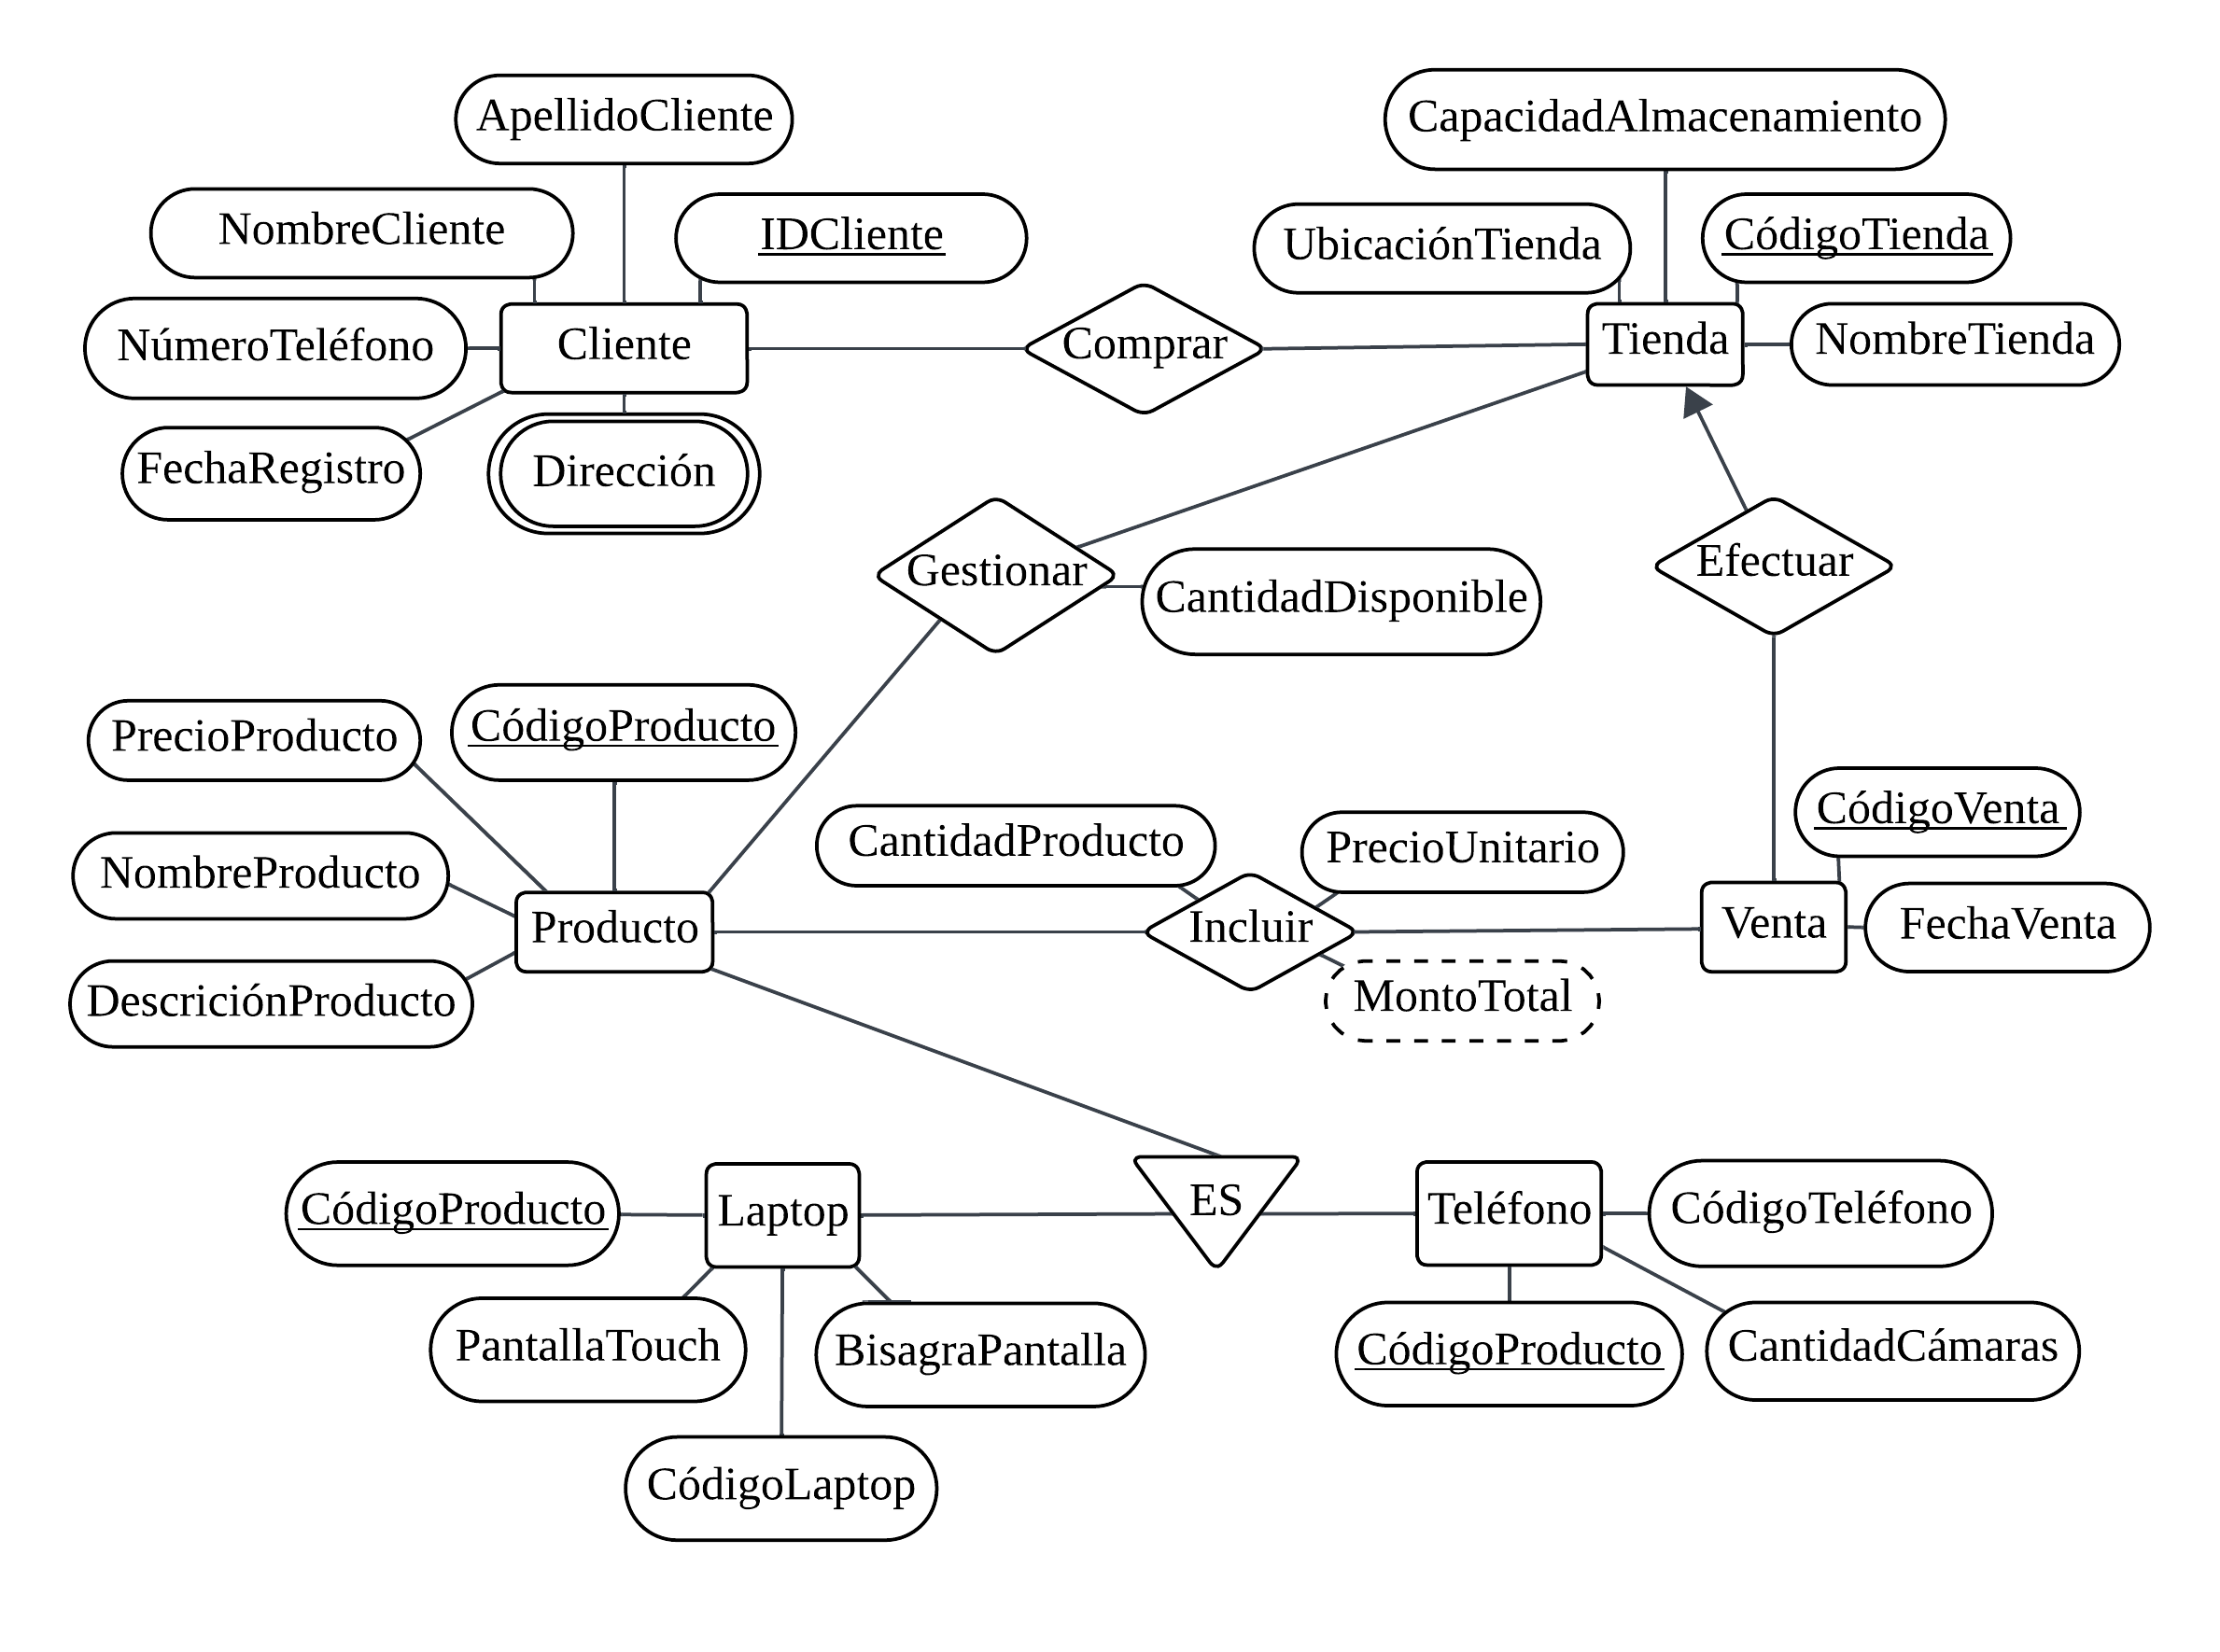
\includegraphics[scale = 0.21]{Imagenes/diagramas/DERE.png}
  \caption{Diagrama Entidad-Relación Extendido}
\end{figure}

\begin{figure}[H]
  \centering
  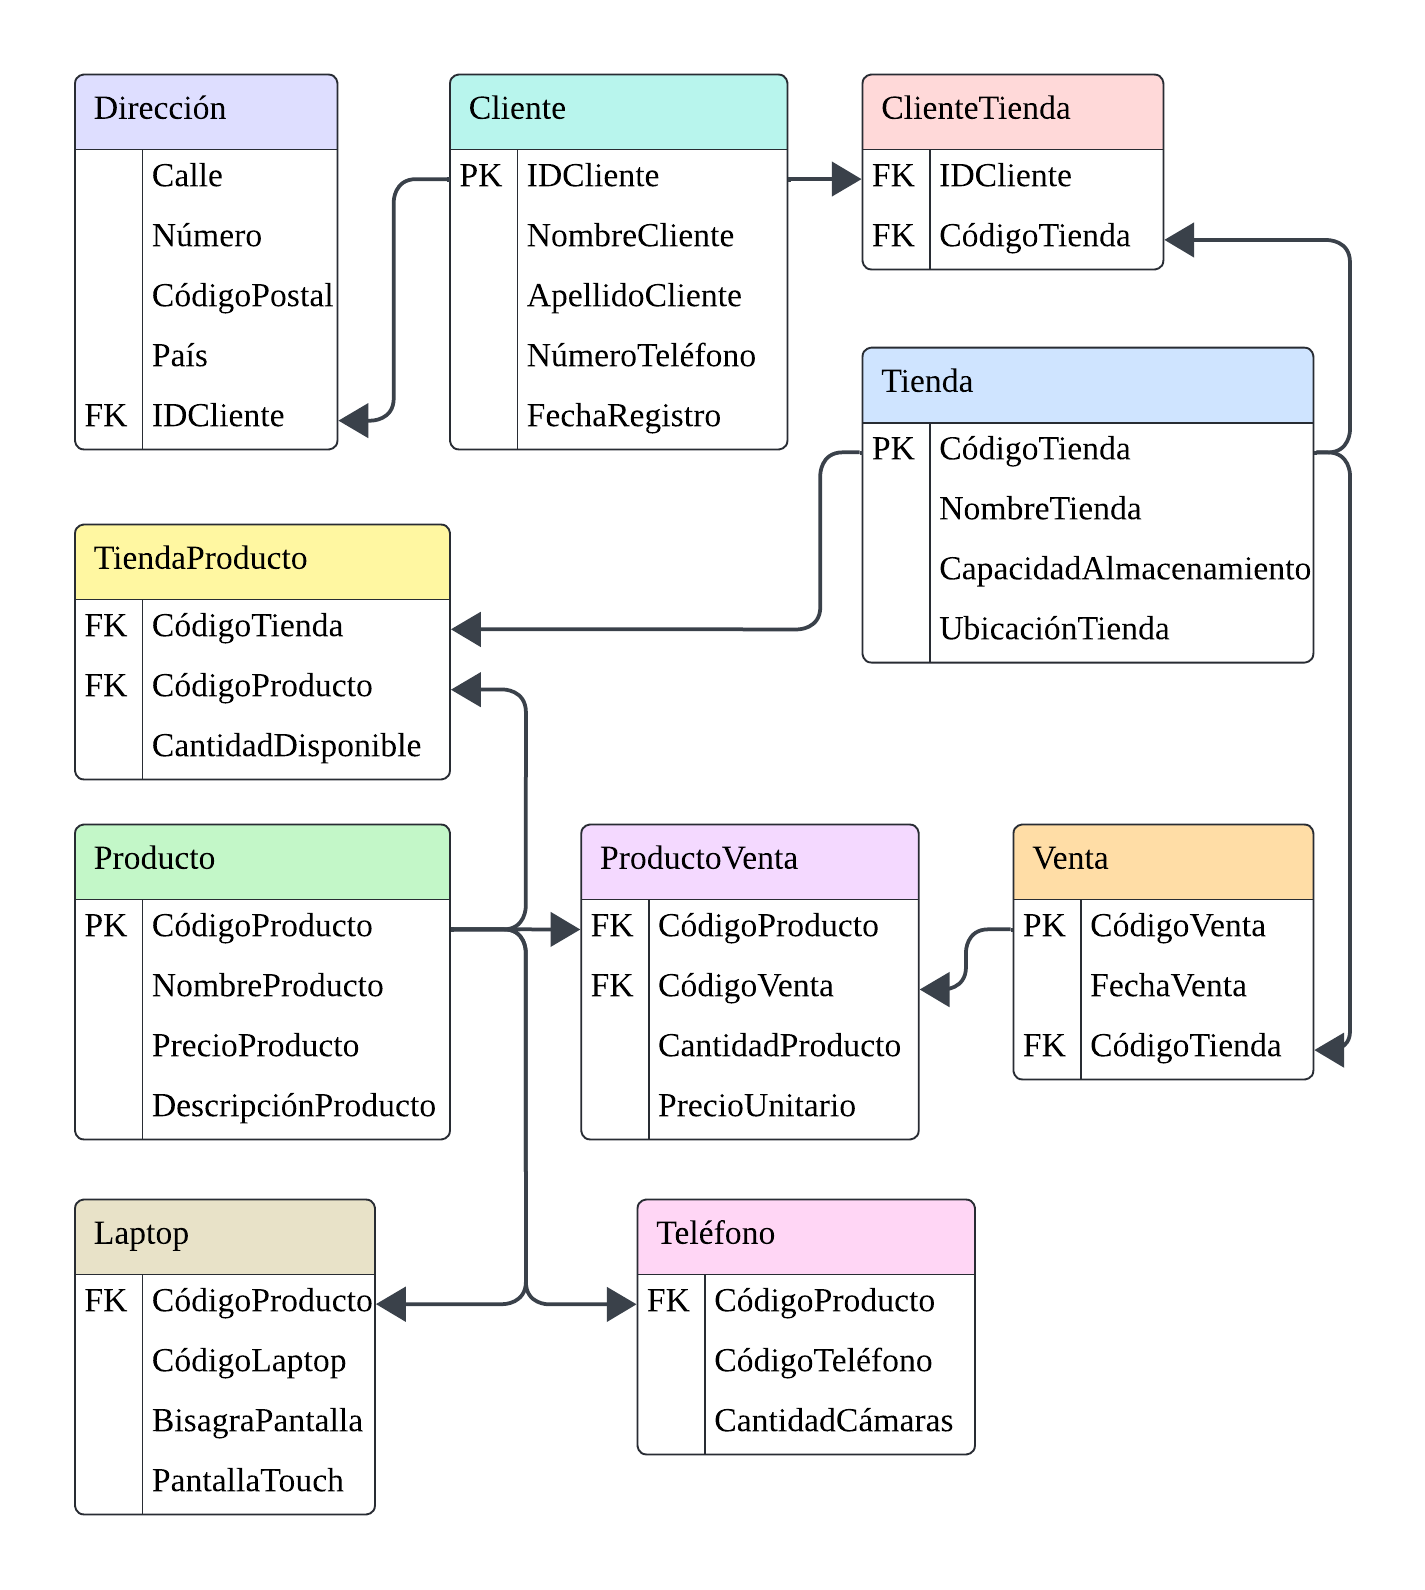
\includegraphics[scale = 0.35]{Imagenes/diagramas/DR.png}
  \caption{Diagrama Relacional}
\end{figure}
\section{Creación}
\begin{figure}[H]
  \centering
  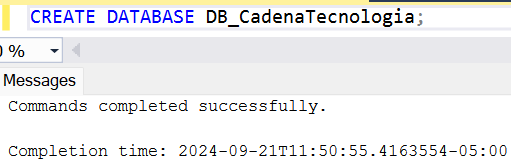
\includegraphics[scale = 1]{Imagenes/sql/1.creacion_db/crear_database.png}
  \caption{Creación de la Base de Datos}
\end{figure}

\begin{figure}[H]
  \centering
  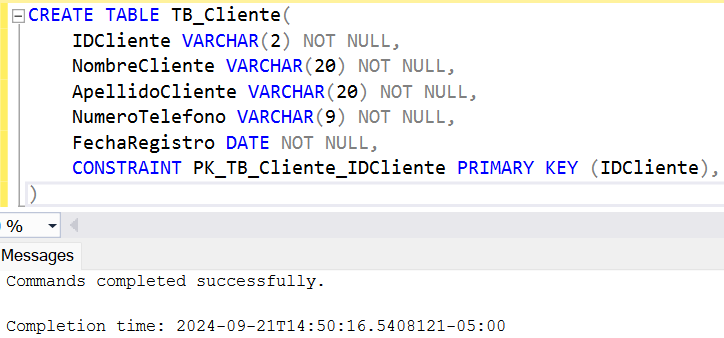
\includegraphics[scale = 0.7]{Imagenes/sql/2.crear_tablas/creacion_tabla_cliente.png}
  \caption{Creación de la tabla Cliente}
\end{figure}

\begin{figure}[H]
  \centering
  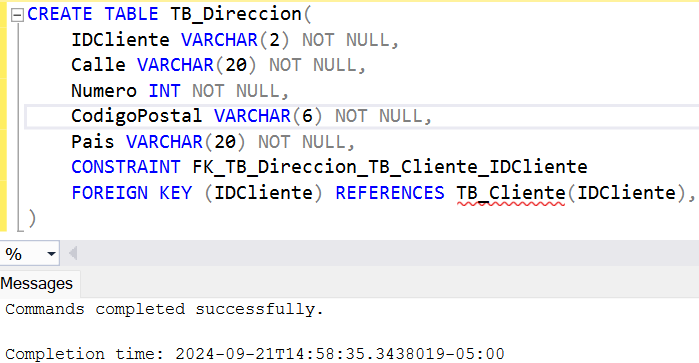
\includegraphics[scale = 0.7]{Imagenes/sql/2.crear_tablas/creacion_tabla_direccion.png}
  \caption{Creación de la tabla Direccion}
\end{figure}

\begin{figure}[H]
  \centering
  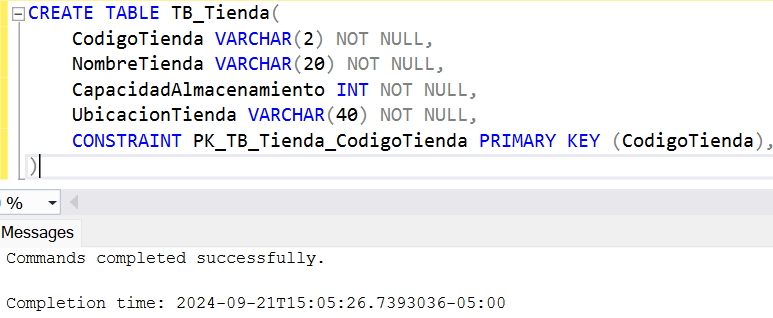
\includegraphics[scale = 0.7]{Imagenes/sql/2.crear_tablas/creacion_tabla_tienda.png}
  \caption{Creación de la tabla Tienda}
\end{figure}

\begin{figure}[H]
  \centering
  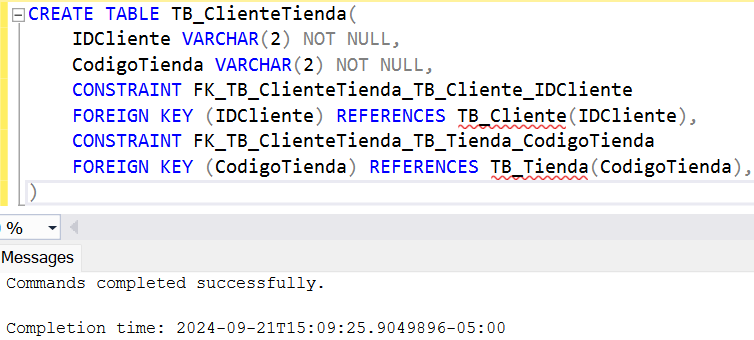
\includegraphics[scale = 0.7]{Imagenes/sql/2.crear_tablas/creacion_tabla_clientetienda.png}
  \caption{Creación de la tabla ClienteTienda}
\end{figure}

\begin{figure}[H]
  \centering
  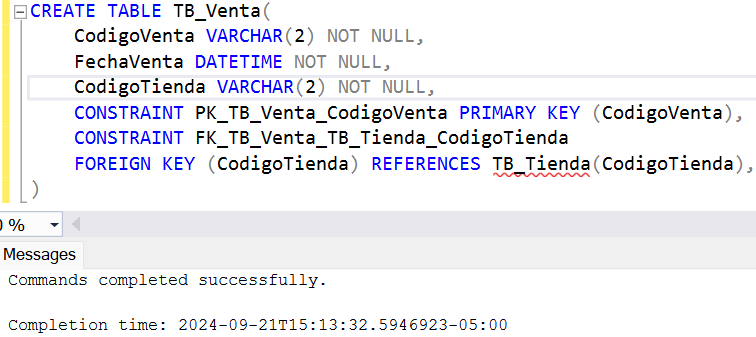
\includegraphics[scale = 0.7]{Imagenes/sql/2.crear_tablas/creacion_tabla_venta.png}
  \caption{Creación de la tabla Venta}
\end{figure}

\begin{figure}[H]
  \centering
  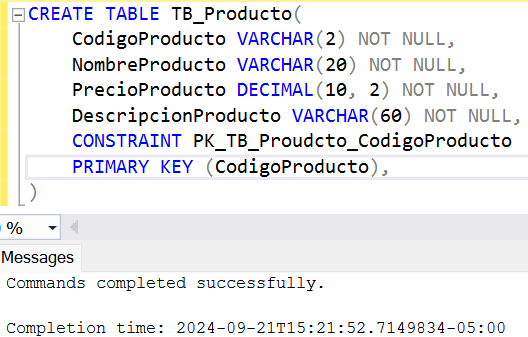
\includegraphics[scale = 0.7]{Imagenes/sql/2.crear_tablas/creacion_tabla_producto.png}
  \caption{Creación de la tabla Producto}
\end{figure}

\begin{figure}[H]
  \centering
  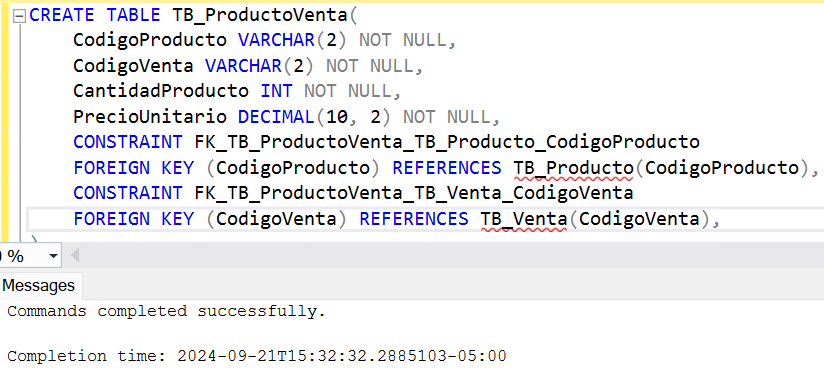
\includegraphics[scale = 0.7]{Imagenes/sql/2.crear_tablas/creacion_tabla_productoventa.png}
  \caption{Creación de la tabla ProductoVenta}
\end{figure}

\begin{figure}[H]
  \centering
  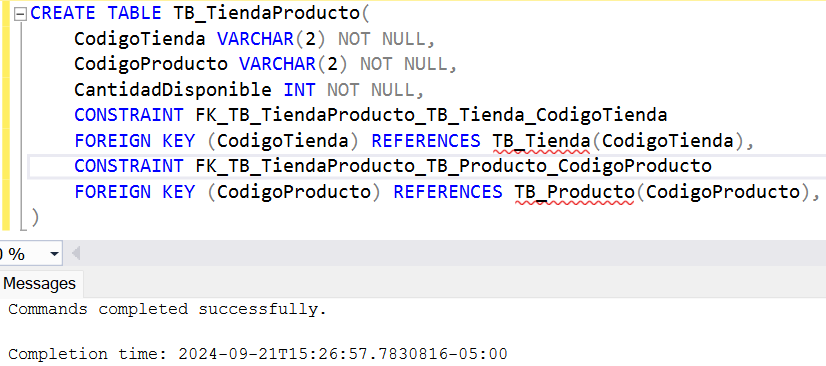
\includegraphics[scale = 0.7]{Imagenes/sql/2.crear_tablas/creacion_tabla_tiendaproducto.png}
  \caption{Creación de la tabla TiendaProducto}
\end{figure}

\begin{figure}[H]
  \centering
  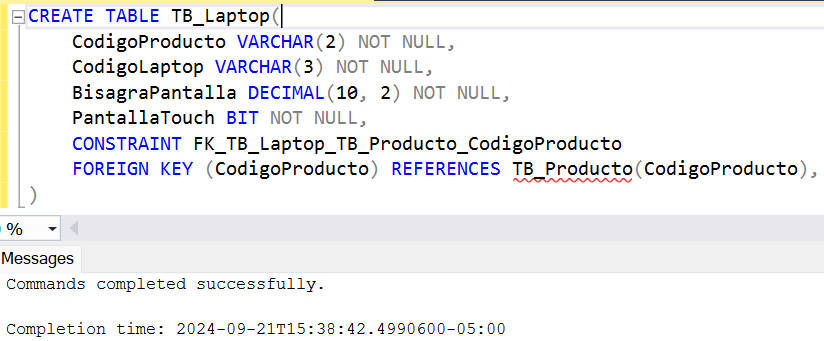
\includegraphics[scale = 0.7]{Imagenes/sql/2.crear_tablas/creacion_tabla_laptop.png}
  \caption{Creación de la tabla Laptop}
\end{figure}

\begin{figure}[H]
  \centering
  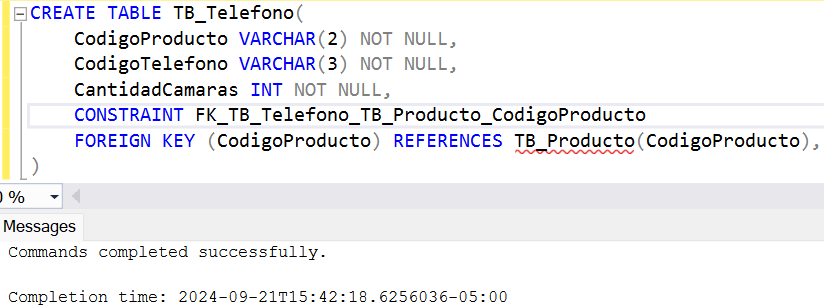
\includegraphics[scale = 0.7]{Imagenes/sql/2.crear_tablas/creacion_tabla_telefono.png}
  \caption{Creación de la tabla Telefono}
\end{figure}


\section{Inserción de registros}
\begin{figure}[H]
  \centering
  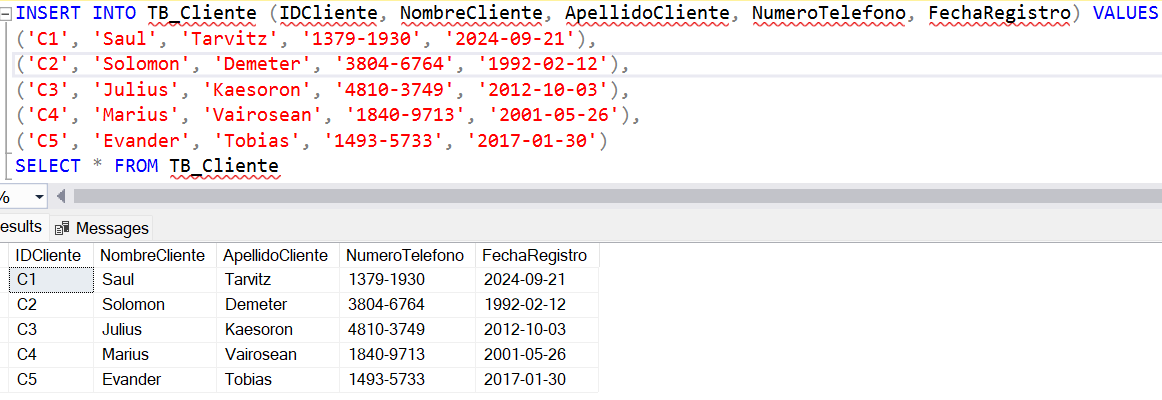
\includegraphics[scale = 0.5]{Imagenes/sql/3.insertar_registros/insertar_registros_cliente.png}
  \caption{Inserción de registros en la tabla Cliente}
\end{figure}

\begin{figure}[H]
  \centering
  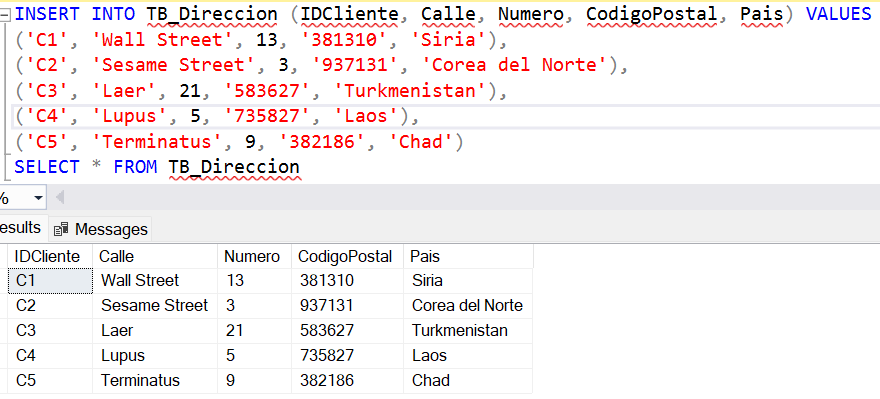
\includegraphics[scale = 0.5]{Imagenes/sql/3.insertar_registros/insertar_registros_direccion.png}
  \caption{Inserción de registros en la tabla Direccion}
\end{figure}

\begin{figure}[H]
  \centering
  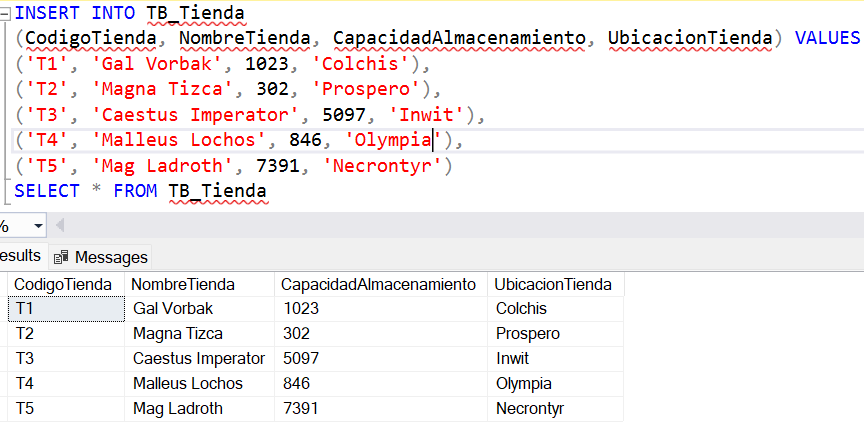
\includegraphics[scale = 0.5]{Imagenes/sql/3.insertar_registros/insertar_registros_tienda.png}
  \caption{Inserción de registros en la tabla Tienda}
\end{figure}

\begin{figure}[H]
  \centering
  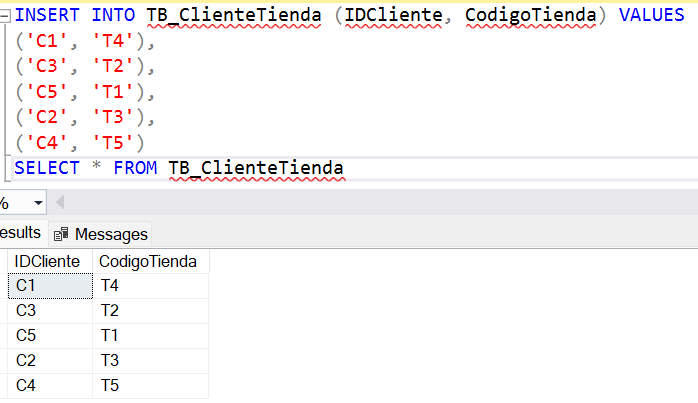
\includegraphics[scale = 0.5]{Imagenes/sql/3.insertar_registros/insertar_registros_clientetienda.png}
  \caption{Inserción de registros en la tabla ClienteTienda}
\end{figure}

\begin{figure}[H]
  \centering
  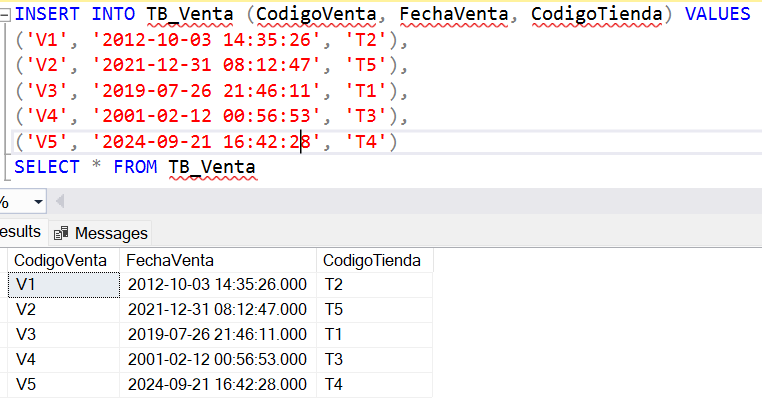
\includegraphics[scale = 0.5]{Imagenes/sql/3.insertar_registros/insertar_registros_venta.png}
  \caption{Inserción de registros en la tabla Venta}
\end{figure}

\begin{figure}[H]
  \centering
  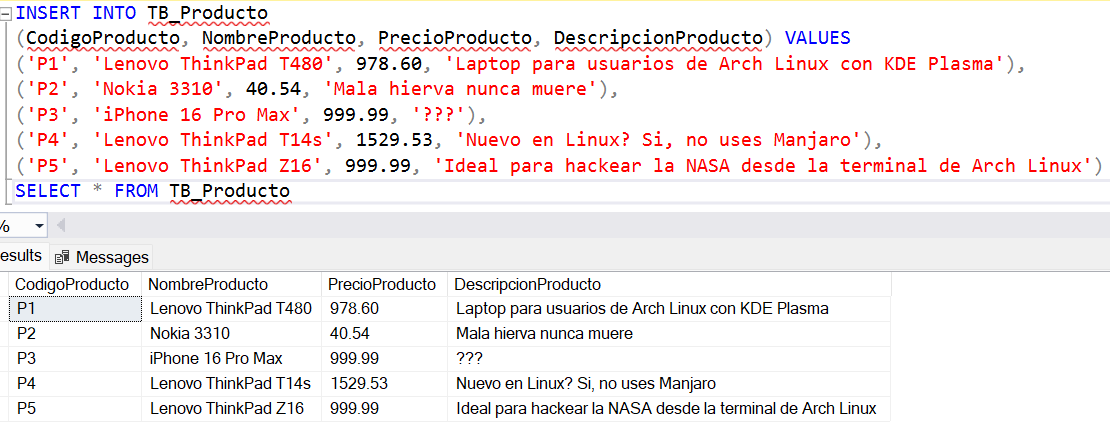
\includegraphics[scale = 0.5]{Imagenes/sql/3.insertar_registros/insertar_registros_producto.png}
  \caption{Inserción de registros en la tabla Producto}
\end{figure}

\begin{figure}[H]
  \centering
  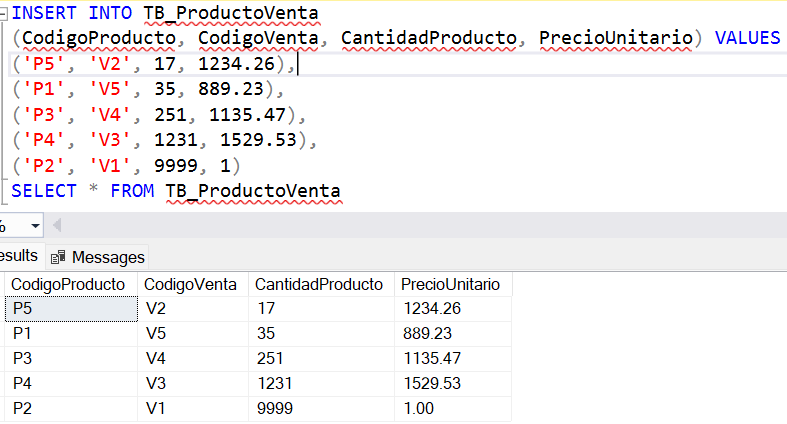
\includegraphics[scale = 0.5]{Imagenes/sql/3.insertar_registros/insertar_registros_productoventa.png}
  \caption{Inserción de registros en la tabla ProductoVenta}
\end{figure}

\begin{figure}[H]
  \centering
  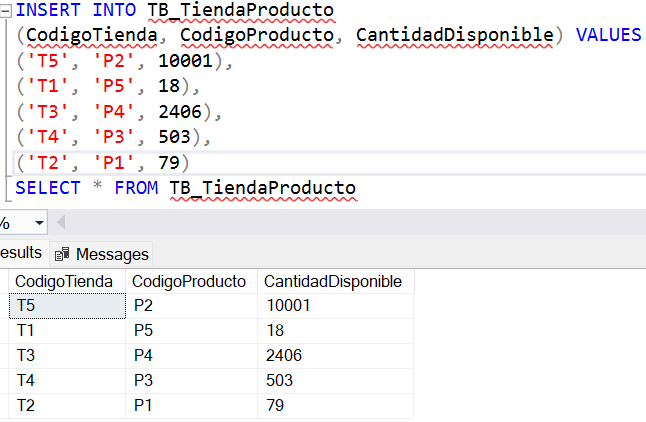
\includegraphics[scale = 0.5]{Imagenes/sql/3.insertar_registros/insertar_registros_tiendaproducto.png}
  \caption{Inserción de registros en la tabla TiendaProducto}
\end{figure}

\begin{figure}[H]
  \centering
  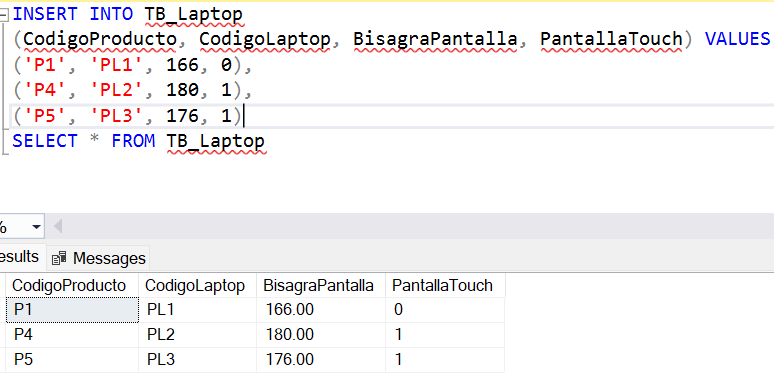
\includegraphics[scale = 0.5]{Imagenes/sql/3.insertar_registros/insertar_registros_Laptop.png}
  \caption{Inserción de registros en la tabla Laptop}
\end{figure}

\begin{figure}[H]
  \centering
  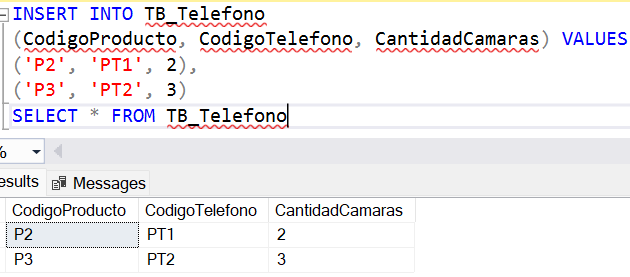
\includegraphics[scale = 0.5]{Imagenes/sql/3.insertar_registros/insertar_registros_telefono.png}
  \caption{Inserción de registros en la tabla Telefono}
\end{figure}
\section{Consultas}
\begin{figure}[H]
  \centering
  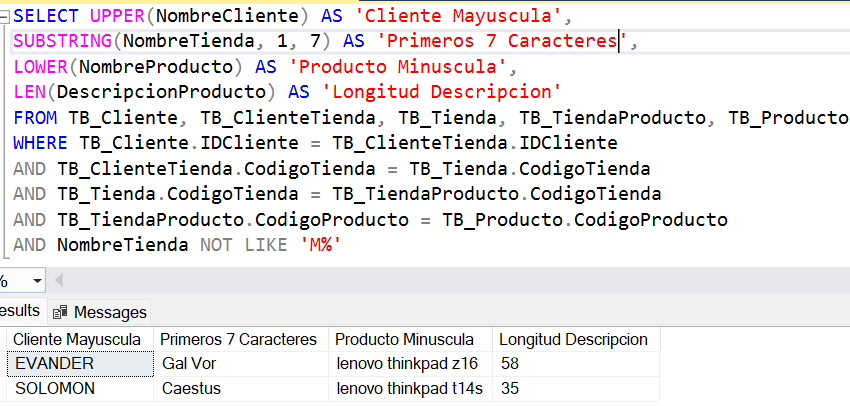
\includegraphics[scale = 0.7]{Imagenes/sql/4.consultas/consulta_cliente_producto.png}
  \caption{Consulta de los Productos que compran Clientes}
\end{figure}

\begin{figure}[H]
  \centering
  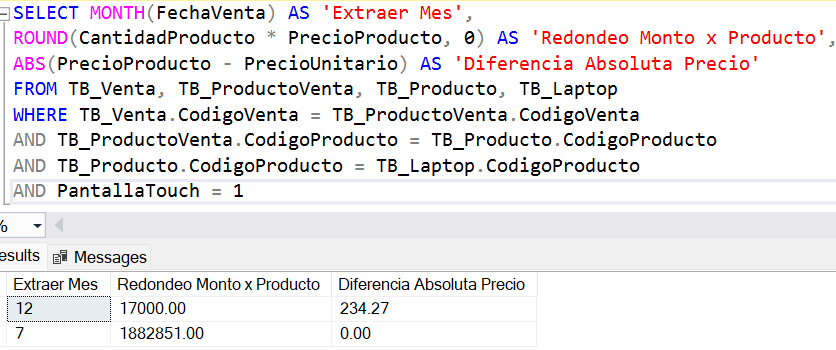
\includegraphics[scale = 0.7]{Imagenes/sql/4.consultas/consulta_venta_laptop.png}
  \caption{Consulta de las Laptops involucradas en Ventas}
\end{figure}
\end{document}